
% This LaTeX was auto-generated from an M-file by MATLAB.
% To make changes, update the M-file and republish this document.

%%% \documentclass{article}
%%% \usepackage{graphicx}
%%% \usepackage{color}

%%% \sloppy
%%% \definecolor{lightgray}{gray}{0.5}
\setlength{\parindent}{0pt}

%%% \begin{document}

    
    
\subsection*{Modified Allan Deviation}

\begin{par}
Example for algorithm MADEV.
\end{par} \vspace{1em}
\begin{par}
MADEV is an algorithm to compute the modified Allan deviation for a set of time-domain frequency data.
\end{par} \vspace{1em}
\begin{par}
See also W. J. Riley, "The Calculation of Time Domain Frequency Stability". Implementation: M. A. Hopcroft, \verb"mhopeng@gmail.com", Matlab Central.'
\end{par} \vspace{1em}

\subsubsection*{Contents}

\begin{itemize}
\setlength{\itemsep}{-1ex}
   \item Generate sample data
   \item Call algorithm
   \item Display results
\end{itemize}


\subsubsection*{Generate sample data}

\begin{par}
A random numbers with normal probability distribution function will be generated into input data \lstinline{DI.y.v}. Next a drift will be added.
\end{par} \vspace{1em}
\begin{lstlisting}[style=mcode]
DI = [];
DI.y.v = 1.5 + 3.*randn(1, 1e3);
DI.y.v = DI.y.v + [1:1:1e3]./100;
\end{lstlisting}
\begin{par}
Lets suppose a sampling frequency is 1 Hz. The algorithm will generate all possible tau values automatically.
\end{par} \vspace{1em}
\begin{lstlisting}[style=mcode]
DI.fs.v = 1;
\end{lstlisting}


\subsubsection*{Call algorithm}

\begin{par}
Use QWTB to apply algorithm \lstinline{MADEV} to data \lstinline{DI}.
\end{par} \vspace{1em}
\begin{lstlisting}[style=mcode]
DO = qwtb('MADEV', DI);
\end{lstlisting}

        \begin{lstlisting}[style=output]
QWTB: no uncertainty calculation
\end{lstlisting} \color{black}
    

\subsubsection*{Display results}

\begin{par}
Log log figure is the best to see modified allan deviation results:
\end{par} \vspace{1em}
\begin{lstlisting}[style=mcode]
figure; hold on
loglog(DO.tau.v, DO.madev.v, '-b')
loglog(DO.tau.v, DO.madev.v + DO.madev.u, '-k')
loglog(DO.tau.v, DO.madev.v - DO.madev.u, '-k')
xlabel('\tau (sec)');
ylabel('\sigma_y(\tau)');
title(['period = ' num2str(DI.fs.v)]);
grid('on'); hold off
\end{lstlisting}

\begin{center}
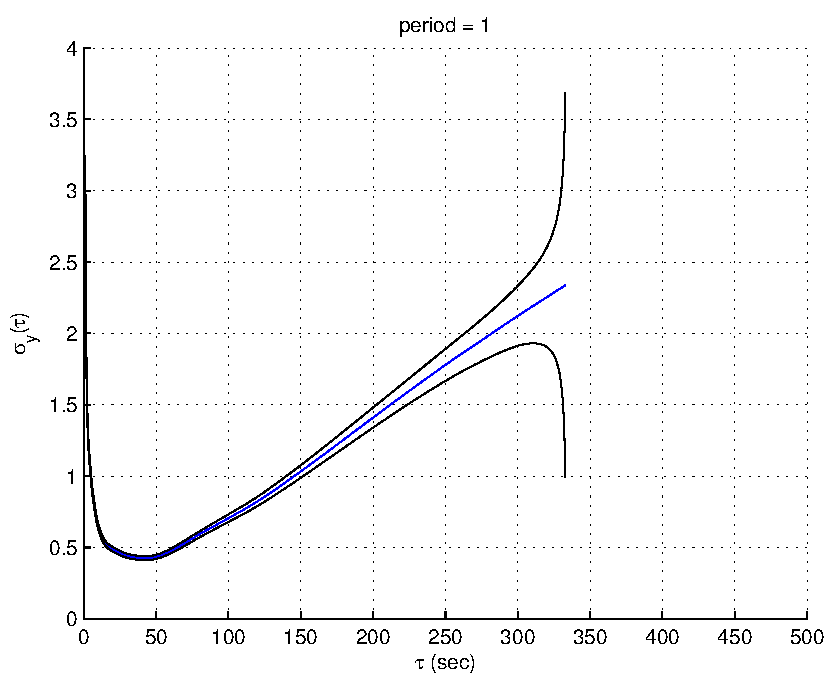
\includegraphics[width=0.7\textwidth]{algs_examples_published/MADEV_alg_example_01.pdf}
\end{center}



%%% \end{document}
    
